\documentclass{aastex62}

\received{September 4th, 2018}

\submitjournal{Drexel University Department of Physics}


%\shorttitle{Sample article}
%\shortauthors{Schwarz et al.}
%\newcommand{\vdag}{(v)^\dagger}
%\newcommand\aastex{AAS\TeX}
%\newcommand\latex{La\TeX}

\begin{document}

\title{CAN A CLOSE ENCOUNTER WITH A SUPERMASSIVE BINARY BLACK HOLE PRODUCE A HYPERVELOCITY GLOBULAR CLUSTER?}

\author{Sean C. Lewis}
\affil{Drexel University Department of Physics \\
Philadelphia, Pennsylvania}



\begin{abstract}

Abstract

\end{abstract}
\section{Introduction} \label{sec:intro}
Astrophysical objects with velocities exceeding 1000 km/s relative to their surroundings are described as  "hypervelocity objects". Of course, any such object is expected to have undergone an extreme gravitational interaction. The most common hypervelocity object directly observed are hypervelocity stars within the Milky Way.  Such objects' possible acceleration mechanisms (gravitational encounters of single stars, tidal disruptions of a stellar binary, and encounters with a binary supermassive black hole) have been explored extensively. In 2014, a comprehensive spectroscopic survey of the massive galaxy M87 noted one particular source to have an extraordinary blueshift compared to the relatively redshifted galaxy \citep{cald14}. The source's emission spectrum was extremely blue-shifted corresponding to a velocity of ~2300 km/s relative to M87. Further analysis of the object's spectra provided modest evidence for the presence of a globular cluster, making it the first directly observed hypervelocity globular cluster, denoted as HVGC-1. Within the paper declaring and supporting HVGC-1's discovery, two possible acceleration methods are proposed along with requests for further analysis through simulation. The first: the globular cluster passed between two separated dark matter potentials. This possibility was addressed briefly in \citet{sam15} and, although further numerical simulations are requested, it will not be explored in this paper. The second possibility: HVGC-1 had a close encounter with a supermassive binary black hole  (SMBBH). It has been proposed that SMBBHs are sources for some of the more extreme hypervelocity objects such as individual stars \citep{yutre03} and intracluster planetary nebulae \citep{hol05}. Although no direct observations of a binary black hole system in M87 has been made, strong evidence exists for the presence of a single supermassive black hole at the galaxy's center \citep{geb11}. In addition, it is presumed that a large galaxy like M87 evolve through mergers (e.g., van Dokkum 2005) and, with supermassive black holes being a standard component of elliptical galaxies and spiral bulges, it is a reasonable assumption that a binary black hole of comparable masses could be present in M87. 

As stated in both \citet{cald14} and \citet{sam15}, there is minimal likelihood that such an encounter could produce an intact globular cluster. It may be the case that, in order to receive a significant velocity kick, the cluster must pass within 10 parsecs of the BBH. Indeed, Caldwell presents scenarios in which a $2*10^6M_{sun}$ cluster passes 2-3 parsecs from the supermassive black hole, an interaction in which the tidal radius on the globular cluster would be 0.3-0.4 pc. Undoubtedly, for a cluster of presumed radius ~6-10 pc, this would be a devastating event, potentially resulting in only the core of the cluster surviving. However, a simple keplerian calculation reveals the time spent in the vicinity of the SMBBH is small, on the order of 5000 years. So, the cluster will experience the extreme tidal forces in the form of nearly a delta function. In addition, if outer stars are being stripped from the cluster, the change in mass may result in a higher exit velocity, making the achievability of "hypervelocity" more reasonable. It is the goal of this paper and analysis to determine the fate of such a globular cluster. 

\section{Creating a simple gravity slingshot}
\subsection{AMUSE Framework}
The Astrophysical Multipurpose Software Environment (AMUSE) is used to accurately model and analyze the behavior of a globular cluster and its constituent stars throughout its close pass with a SMBBH. AMUSE uses an integrator to evolve a gravitational system while also allowing the user to pause said integration and record data such as particle mass, position, velocity, and energy. I chose to use the N-body integrator ph4. Although I initially investigated a simple system of 3 point-particles, the use of ph4 would become necessary once the globular cluster particle was expanded to include {\raise.17ex\hbox{$\scriptstyle\mathtt{\sim}$}}1000 stars. 

\subsection{Initial Conditions}
As stated in the previous subsection, I began my simulation construction by generating and evolving a simple 3-body interaction. Two of the bodies acted as the supermassive black holes: each were given an appropriate mass and orbit parameters based on user defined total mass, mass ratio, and constant separation distance. This binary system was simplified into a nested set of circular orbits. The initial position and velocity vector components of the black hole particles were calculated with basic orbital mechanics and trigonometry. I will refer to the "phase" of the black holes throughout this paper. If both black holes were placed along the x-axis at the beginning of integration, the black holes are said to have a phase of 0 radians. A phase of $\pi$ radians corresponds to the black holes lying on the y-axis. The code also places a globular cluster particle at a distance of {\raise.17ex\hbox{$\scriptstyle\mathtt{\sim}$}}120 parsecs away from the black hole binary in the same plane as the binary orbits. The distance is an estimate because, in addition to being initially displaced from the SMBBH by set 100 pc along the y-axis, the GC is offset along the x-axis by the impact parameter of the interaction. The impact parameter is calculated by examining the conservation of energy and angular momentum of the globular cluster as it travels from "infinity" to its closest approach to the black holes:
\begin{equation}
\frac{1}{2}v_{\infty}^2 = \frac{1}{2}v_{c}^2 - \frac{GM_{BH}}{r_{c}}
\end{equation}
\begin{equation}
L = v_{\infty}b = v_{c}r_{c}
\end{equation}
\begin{equation}
b = r_{c}\sqrt{1+\frac{GM_{BH}}{r_{c}v_{\infty}^2}}
\end{equation}
Where $v_{\infty}$ is the GC initial velocity far from the black hole binary, $v_{c}$ is the GC velocity at closest approach, G is the gravitational constant, $M_{BH}$ is the total mass of the black hole binary, $r_{c}$ is the GC's closest approach to the BBH center of mass, and b is the impact parameter.  In addition, an unvaried $v_{\infty}$ and $M_{BH}$ were chosen as 500 km/s and $7 \times 10^9 M_{\odot}$ respectively. So, by asserting a distance of closest approach, AMUSE will generate a simulation in which the GC falls towards the SMBBH, undergo a prograde planar interaction, and then have the GC's ejection velocity recorded once it reaches 120 pc away from the BBH. 

\subsection{Mirroring HVGC-1}
By examining the galactic potential of M87, a rough estimate can be made for the necessary ejection velocity of an object recorded at 120 pc from the galactic center in order to possess a velocity of 2300 km/s at a significantly further radial distance. Assuming a power-law density model where the mass density behaves as $\rho(r) = \rho_{o}(r_{o}/r)^\alpha$ and the mass within radius r is $M(r) = (4\pi G\rho_{o}r_{o}^\alpha r^{3-\alpha})/(3-\alpha)$, the potential difference at two different radii can be calculated:
\begin{equation}
\Phi(r) - \Phi(r_{o}) = G\int_{r_{o}}^{r} \! \frac{M(r')}{r'^2} \, \mathrm{d}r' = \frac{4\pi G\rho_{o}r_{o}^\alpha }{3-\alpha} r^{3-\alpha}\int_{r_{o}}^{r} \! r'^{1-\alpha} \, \mathrm{d}r'
\end{equation}
We take $\alpha$ to be equal to 2 under the assumption the mass density of the galaxy is proportional to $r^{-2}$. This is acceptable for this order-of-magnitude estimation, although it has been noted that more complicated multi-moment potentials may be present in and around M87 \citep{mur14}. So,
\begin{equation}
 %= \frac{v_{c}^{2}(r_{o}) - v_{c}^{2}(r)}{\alpha - 2} for \alpha \neq 2
 \Delta\Phi= v_{c}^{2}ln(r/r_{o})
\end{equation}
Where $v_{c}$ is the circular velocity, which I take here to be equivalent to the velocity dispersion of M87: 500 km/s, r is the distance from M87 at which HVGC-1 is thought to be, $\gg$85 kpc, and $r_{o}$ is the distance from the galactic center at which my simulation ends and records an ejection velocity, 120 pc. By setting the change in kinetic energy equal to equation 5, we find the ejection velocity at 120 pc to be:
\begin{equation}
v_{o} = \sqrt{v_{r}^2 + 2v_{c}^{2}ln\bigg(\frac{r}{120 pc}\bigg)}
\end{equation}
%\begin{figure}
%\figurenum{1}
%\plotone{./Images/velocity_behavior.png}
%\caption{text}
%\end{figure}
\begin{figure}
\figurenum{1}
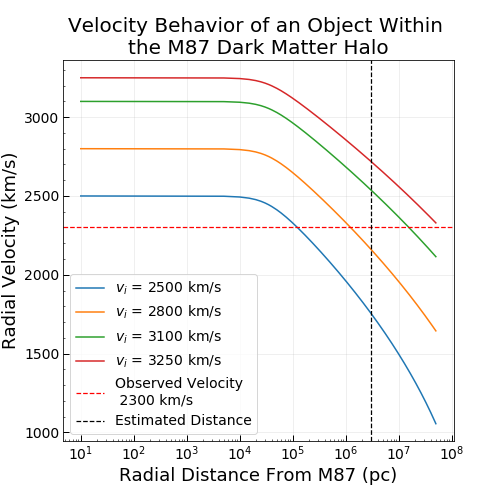
\includegraphics[scale=0.7]{./Images/velocity_behavior.png}
\centering
\caption{text}
\end{figure}
Based on my rough estimation of the potential well of M87, an object's exit velocity (recorded in my simulation at 120pc away from the SMBBH) on the order of 3000 km/s is necessary for an observed velocity of 2300 km/s at the estimated distance of HVGC-1. Any exit velocity less than {\raise.17ex\hbox{$\scriptstyle\mathtt{\sim}$}}2100 km/s will result in the object being incapable of reaching a distance of 1Mpc, and will be still bound to M87. I will explore parameters of the binary black hole system that will permit a significant exit velocity as well as examine specific scenarios that will allow for a star cluster to survive the interaction and exhibit velocities similar to those observed in \citet{cald14}.
\subsection{Cluster Exit Velocity and BH Phase Dependence}
The cluster's exit velocity depends heavily on the location of the black holes during its closest approach to the binary. In order to determine the ideal location of the BH's during the interaction, the simulation was repeated while varying the initial phase of the black holes. This is analogous to varying the BH phase during closest approach. The result: a BH phase dependent exit velocity that clearly shows two peaks corresponding to the cluster arriving at the SMBBH while the outer and inner BH are in phase with it, see Figure 1.
%\begin{figure}
%\figurenum{1}
%\plotone{./Images/phase_loop_curated.png}

%\caption{text}
%\end{figure}
Interestingly, some BH phases result in the test particle becoming captured by the binary black hole system. An easy check to confirm a gravity capture is taking place (as opposed to some odd unintended consequence within the AMUSE code) is to investigate the test particle's energy during the interaction. It would be expected that the particle's total energy relative to the center of mass of the system is a conserved quantity, that is, until a close pass with the SMBBH whereafter the particle's energy will be lower. Indeed, this is what is observed, see Figure 2. For comparison, an interaction that results in the ejection of the GC will have the GC's relative energy also remain constant as it infalls towards the SMBBH, then have a positive shift after the interaction, see Figure 3. Interactions that result in a captured GC test particle were discarded and not considered further as this investigation focuses only on the possibility of a GC being ejected at greater than 1000 km/s, but such interactions may be useful for further simulations regarding stellar or more complex structure capture by binary black holes.

\begin{figure}
\figurenum{2}
\plottwo{./Images/bound_track.png}{./Images/bound_energy.png}

\caption{Left: The globular cluster (red path) begins its path at the bottom right at (38 pc, -100 pc) and begins infalling towards the black hole binary (black path: more massive BH, blue path: less massive BH. Notice how the GC appears to be tracing a path that is beginning to turn back around towards the SMBBH. Right: The relative energy, in Joules, of the globular cluster during throughout its journey towards, around, and away from the SMBBH. The oscillation and large spike are due to the gravitational potential close to the SMBBH becomes more significantly more complex than the assumed point mass viewed from infinity. Here, the GC begins at -3.15E48 J of relative energy and ends with -4.42E48 J, a 40.3\% decrease in energy relative to the center of mass of the system.}
\end{figure}

\begin{figure}
\figurenum{3}
\plottwo{./Images/unbound_track.png}{./Images/unbound_energy.png}

\caption{Left: All initial conditions are equal to those in Figure 1 except for the location of the black holes in their orbit during the GC's closest pass. Notice, the GC (red line) makes a much more direct path away from the SMBBH than in Figure 1. Right: After its interaction with the SMBBH, the GC has gained relative energy and has been ejected from the system. Here, the GC begins with -3.15E48 J of energy (the same as in Figure 1) and ends with +1.94E48 J, a 161.6\% increase in energy.}
\end{figure}
\subsection{Operational Parameters}
So, the operational parameters of this prograde planar interaction were BH mass ratio, the separation of the BHs, the GC's closest approach, and BH phase. These values were varied to explore the parameter space in an attempt to determine the combination that resulted in the highest GC exit velocity and smallest tidal perturbation: $\gamma = {a_{t}}/{a_i}$ where $a_{t}$ is the tidal acceleration of the GC due to the presence of the external BH gravity well and $a_{i}$ is the internal acceleration of the GC. A small tidal perturbation implies a higher likelihood of a significant fraction of the star cluster surviving the interaction. To explore a large range of parameter space, the following were chosen: BH mass ratio [0.01, 0.05, 0.1, 0.25], BH Axis (pc) [1.7, 3.0, 5.0], GC closest approach (number of times greater than the BH Axis) [1.5, 2, 2.5]. With each combination of parameters, the interaction was repeated with initial BH phases varying by steps in $\pi/15$ such that the most optimum orientation of the BHs can be isolated and investigated further. 

\subsection{Optimum Interaction}
In total, 1,080 simulations were run and only 147 resulted in an GC test-particle exit velocity exceeding 1000 km/s, satisfying the "hypervelocity" condition. Each interaction also recorded the tidal perturbation experienced. Of the 147, I chose three that were of particular interest, see Table \ref{results}. The first interaction listed has the highest velocity to tidal perturbation ratio out of all of the interactions, meaning the largest test-particle exit velocity and the smallest tidal perturbation experienced. The second interaction listed has the highest velocity to perturbation ratio for an event resulting in a velocity $>$2000 km/s. The third has the highest ratio for an interaction with a $>$3000 km/s exit velocity. Notice, all three interaction involve a BBH mass ratio of 0.25, as did the majority of the 147 hypervelocity interactions (63$\%$). In fact, there were zero interaction that resulted in a hypervelocity exit by the test particle for a BH mass ratio of 0.01. A higher mass ratio allows the GC to receive a substantial velocity kick while remaining further away from the black hole binary, resulting in a lower tidal perturbation.  Although, to describe the tidal perturbation as "low" would be to misrepresent the nature of the encounter. Even in the ideal scenario (the first interaction in Table \ref{results}), the tides experienced by the GC due to the presence of BH masses $M_{1}$ and $M_{2}$ reach a respective maximum at 650 and 693 times the internal acceleration of the star cluster. This highlights the extraordinary nature of the encounter, and implies that the cluster will almost certainly be torn apart unless the tidal ratio remains high for a brief enough time period. The encounter that is most capable of mirroring HVGC-1's current behavior is the third entry in Table \ref{results}, where the star cluster briefly experiences a tidal acceleration 67,621 times its internal acceleration. These two interactions were chosen for further analysis as the first satisfies the condition of the production of a hypervelocity object, and the second satisfies initial velocity conditions necessary for HVGC-1's extraordinary behavior. The "ideal-ness" of these three encounters can be refined in the future. However, in my opinion, doing so would reduce an already unlikely scenario down to a near impossible set of perfect circumstances. For the purposes of determining the survivability of a star cluster, these "ball-park" parameters will suffice. 
\subsection{Comparison to HVGC-1}
The object highlighted in \citet{cald14} was determined to be traveling at {\raise.17ex\hbox{$\scriptstyle\mathtt{\sim}$}}2300 km/s outwards from M87 at a distance of 84 kpc
\begin{table}
\centering
\caption{Interactions of interest. Columns from left to right: Exit velocity of the GC 120 pc away from the BBH, mass ratio of the black holes, BH separation distance, Minimum distance from the binary center of mass achieved by the GC, Initial BH phase, Maximum tidal perturbation experienced by the GC due to $M_{1}$ (more massive component), Maximum tidal perturbation due to $M_{2}$. \label{results}}

\begin{tabular}{ccccccc}
\hline \hline
Velocity (km/s) & $M_{2}/M_{1}$ & BH Axis (pc) & Min Dist. (pc) & BH $\Phi$ (rad) & $\gamma_{1}$ & $\gamma_{2}$  \\
1124 & 0.25 & 5.0 & 8.5 & 5.24 & 650 & 692 \\
2336 & 0.25 & 3.0 & 4.5 & 4.61 & 4771 & 7768 \\
3436 & 0.25 & 1.7 & 2.5 & 1.47 & 28584 & 67621 \\
\end{tabular}
\end{table}

\section{A Close Pass of a GC with a SMBBH}
To determine a cluster's ability to survive, the test particle must be extended to a self-gravitating particle cluster.  and reasserting the ideal parameters determined  repeating the 

\begin{thebibliography}{}
\bibitem[Caldwell et al.(2014)]{cald14} 
Caldwell, N., Strader, J., Romanowsky, A. J., et al. 2014, \apjl, 787, L11
\bibitem[Gebhardt et al.(2011)]{geb11}
Gebhardt, K., Adams, J. Richstone, D., et al. 2011, \apj, 729, 13
\bibitem[Holley-Bockelmann et al.(2005)]{hol05}
Holley-Bockelmann et al. 2005, \apjl
\bibitem[Murphy, J., Gebhardt, K., Craidt, M.(2014)]{mur14}
Murphy, J., Gebhardt, K., Craidt, M. 2014, \apj
\bibitem[Sesana et al.(2008)]{ses08}
Sesana, A., Haardt, F., Madau, P. 2008, \apj, 686
\bibitem[Samsing(2015)]{sam15}
Samsing, J. 2015, \apj, 799, 11
\bibitem[Yu \& Tremaine(2003)]{yutre03}
Yu \& Tremaine. 2003, \apj, 599
\end{thebibliography}
\end{document}
